%!TEX root = ../Thesis.tex
\chapter{Introduction to tools of supervised machine learning}

\section{Supervised machine learning to predict and to learn}
Supervised machine learning is either regression, classification or probability estimation models built on labeled data. Regression is to predict scalars (numbers), classification to predict class membership or lastly to rather predict a probability distribute across class. The direct motive of supervised modeling is to predict a certain target information of a given object, that is otherwise expensive/tedious to measure, or only reveal it self in the future, or the measuring is invasive and will destroy the object of interest. The target is predicted by learning a simple or perhaps complex relationship between easy accessible feature information and the target from a labeled training data set. When a useful relationship has been established with a model, target predictions can be made for a unlabeled data set without the target information. A indirect motive of supervised machine learning, is to elucidate the relationship between features and target. One example of an indirect motive, is when modeling the contraceptive method choice reference data set \cite{welling2016forest,lichman2013uci}. Here, +1000 Indonesian married women had answered a questioner on contraception and socio-economic status. To build a model to accurately predict contraception method choice based on 10 questions on socio-economic status was never the actual motive, as it has little practical use to ask 10 questions to only estimate one answer. Why not just ask the right question once? However, the structure of an accurately predicting model can be a useful empiric proposal for a general relationship in society. Scientificly, the next step is then to form a testable causal link theory based on the observed relationship.

\begin{figure}
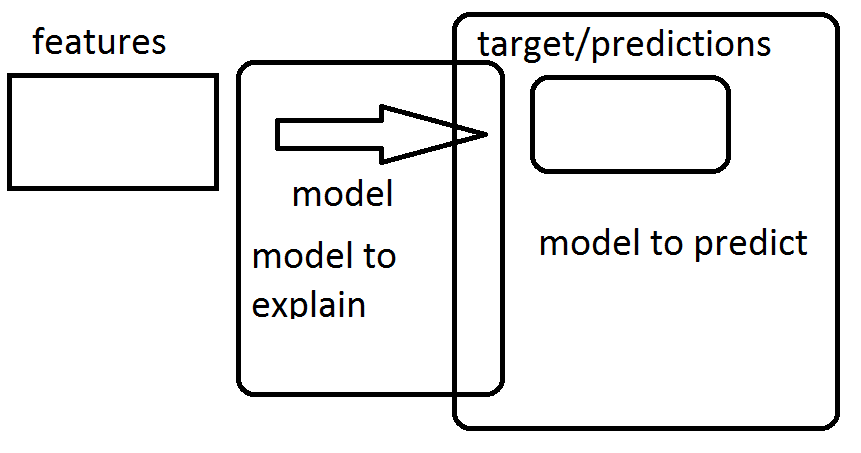
\includegraphics[width=\textwidth,height=\textheight,keepaspectratio]{graphics/modelPredictExplain.png}
\caption{A supervised model learn a relationship between observed features and targets and produce predictions. In order to predict most accurately a robust model with a low prediction error is sought for. One can also use supervised modeling to explore the possible relationship between features and targets, here the question is what is the structure of models providing accurate and robust predictions?}
\label{modelPreditExplain}
\end{figure}

A typical labeled data set, is organized as a data table with one column with desirable target information and a series of columns with feature information. Every row is an independent observation of one target and features. A practical example is the public abalone data set. Here, a marine biologist may be interested in estimating the age of abalones (shellfish). However, determining age is tedious and requires to sacrifice each specimen to study the broken shell under a microscope after chemical staining. To measure the size and weight and to observe the gender is in contrary easy \cite{lichman2013uci}. Therefore the marine biologist can use a supervised regression model to learn a relationship between morphology and age, and use the this relationship to predict effortless the age of new specimens.

\subsection{Univariate Regression}
Perhaps a single feature such as weight ($x_{.1}$) would be almost perfectly linear related to age ($y_.$). In such case uni-variate linear regression (ordinary least squares) would be a sufficient model. Where $\hat{y} = b_1 x_{.1} + b_0$, and where $b_1$ and $b_0$ are chosen to minimize a loss function evaluating the training error. Let $x_{.1}$ be a vector of weight measurements for abalone in training set and let $y_.$ be a vector target measurements, age. Both $x_.1$ and $y_.$ are of length $N$, the sample size of the training set, and the elements are enumerated from $1$ to $N^{th}$ observation by $i$, such that $y_i$ is the age of the $i^{th}$ abalone, and $x_{i1}$ is the weight.

Perhaps the abalones growth rate increases with age, and therefore the age of larger abelones is in general overestimated. To overcome this the model my be manually expanded with a quadratic term such that $\hat{y} = b_2 x_{.1}^2 + b_1 x_{.1} + b_0$. By plotting the relationship and inspecting the residuals it was obvious that linear fit was not optimal. Thus in this manual approach, first a linear fit was made, and by inspecting the residuals it was obvious that transforming the weight measurements by non-linear quadratic transfer function would improve the linear relationship.

\subsection{Multiple linear regression and interaction terms}
The user may now start to include several transposed features and interaction terms and to an extend where the number of input features in the regression model even outnumbers the number of observations. Thus there is no direct limitation in linear regression to not model non-linear relationships and interactions terms, all these terms just have to be stated manually. For a small set of features, and where the goodness-of-fit of a linear model is already fair, it is easy to inspect the residuals to observe how a linear fit may be inadequate. Hereafter one can specify some useful transfer functions and interactions terms and obtain a even better model. One the number of features become larger

One limitation is the degrees of freedom. In a linear ordinary least squares model, if the number of parameters in the model outnumbers the number of observations, there is no longer one unique with a minimal loss function score, but rather a subset of solutions all with no error. It takes only an offset and a slope to connect two points with a line, or an offset and two slope coefficents to describe a plane connecting three points. Likewise, 18 points can always be connected by an 17-dimensional hyper plane plus an offset.

The accuracy of a model should not be evalauted by training error epescially, when then number of parameters are close to as many observations and/or if the observations are noisy.

Psychologist and economist Daniel Kahneman noted when working with notoriously noisy data from psychology tests, that multiple linear regression models explained the training data well, however the established model predicted poorly future results and could not be reproduced. Each subject would be exposed to a number of tests and instead of estimating a coefficient to each partial test he much preferred to use the summed total score as a predictor, thus giving each sub test the same weight. He found this approach more accurate and reproducible than multiple linear regression\cite{kahneman2011thinking}. What Kahneman in practice performed here is called regularization, although a relatively crude version. A more elegant regularization method ridge coefficient estimator \footnote{A special case of elastic-net. Elastic-net is a linear combination lasso and ridge, both estimating a squared coefficent penelization norm (L2/lambda) and a absolute sum norm (L1/alpha). L1 norm tend to drive features towards zero, and can be used for combined regularization and feature selection} is defined as 

\begin{equation}
2+2


\end{equation}



\begin{quote}
"With four parameters I can fit an elephant, and with five I can make him wiggle his trunk"  - John von Neumann
\cite{wiki2016John}
\end{quote}


training eror versus test error. Approximation future model accuracy.
Assumptions cross-validation
sand-boxing models




\subsection{Feature selection}
A crude solution is to univariatly filter any feature or interaction term, that do not have a linear relationship (e.g. pearson correlation) above a certain threshold.



\subsection{Feature selection and Regularization}


\subsection{Algorithmic models}
So far multiple linear regression have worked well even for non-linear problems, if the operator can come up transfer functions which output relate linearly to the target. However, for multivariate data set, where an initial multiple linear regression model has a low goodness-of-fit, it can be very difficult to decide from residuals plots by each variable, what series of transfer function and interaction terms would improve the model. The residuals may even seem to follow a normal distribution, even though the ideal underlying function generating the data is non random. Algoritmic models are loosly defined as defined in algorithms, rather than mathematical expressions. However, any algorithm can be likely be expressed in a mathematical expression, it may just perhaps a very incomprehensible one. Popular algorithm models presently are radial basis support vector machine (RB-SVM), $k^{th}$-nearest neighbor (kNN), random forest (RF), gradient boosting trees (GBT) and neural nets (NN). An introduction to each type of model is beyond the scope of this thesis and especially neural nets has today a large field special tailored for the purpose sub-models, such as convolutional nets, recurrent nets, deep layered nets or any combination of these. From a user view point, all these algorithmic models have in common that features can inputted without specifying transfer functions, and the model will automatically to some extend fit non-linear relationships, interactions, provide regularization and robustness to outliers. A given algorithmic models should be considered instead, whenever this seem out perform linear regression in cross-validated prediction error.

